% =====================================================================
%  V2V-Project -- Study Pack
%  Section S3 : The Cryptographic Core
%  Source file studied: crypto/crypto.py
%  Standalone document -- compile with:  pdflatex 03-cryptographic-core.tex
% =====================================================================
\documentclass[11pt,a4paper]{article}

\usepackage[utf8]{inputenc}
\usepackage[T1]{fontenc}
\usepackage{lmodern}

\usepackage[a4paper,margin=2.4cm]{geometry}
\usepackage{enumitem}
\setlist{topsep=2pt,itemsep=2pt}

\usepackage{amsmath}
\usepackage{amssymb}
\usepackage{booktabs}
\usepackage{graphicx}
\usepackage{xcolor}
\usepackage{listings}
\usepackage{tikz}
\usetikzlibrary{arrows.meta,positioning,shapes.geometric,calc,fit,backgrounds}
\usepackage[colorlinks=true,linkcolor=blue,urlcolor=blue,citecolor=blue]{hyperref}

\definecolor{codebg}{rgb}{0.97,0.97,0.94}
\definecolor{codegreen}{rgb}{0.00,0.50,0.00}
\definecolor{codegray}{rgb}{0.50,0.50,0.50}
\definecolor{keyblue}{rgb}{0.00,0.20,0.70}
\definecolor{boxblue}{rgb}{0.88,0.93,1.00}
\definecolor{boxyellow}{rgb}{1.00,0.97,0.85}

\lstdefinestyle{py}{
  language=Python,
  backgroundcolor=\color{codebg},
  basicstyle=\ttfamily\footnotesize,
  keywordstyle=\color{keyblue}\bfseries,
  stringstyle=\color{codegreen},
  commentstyle=\color{codegray}\itshape,
  numberstyle=\tiny\color{codegray},
  numbers=left,
  numbersep=8pt,
  showstringspaces=false,
  breaklines=true,
  breakatwhitespace=false,
  frame=single,
  rulecolor=\color{codegray},
  tabsize=4,
  captionpos=b,
}
\lstdefinestyle{term}{
  backgroundcolor=\color{codebg},
  basicstyle=\ttfamily\footnotesize,
  breaklines=true,
  frame=single,
  rulecolor=\color{codegray},
  numbers=none,
  captionpos=b,
}

\title{\textbf{V2V-Project Study Pack}\\[4pt]
       \large Section S3 --- The Cryptographic Core\\
       \large \normalsize AES-256-GCM, ECDH, HKDF, ECDSA}
\author{Information Security Project --- Beginner Study Notes}
\date{Source file: \texttt{crypto/crypto.py}}

\begin{document}
\maketitle
\tableofcontents
\newpage

% =====================================================================
\section{Title and ``What You'll Learn''}
% =====================================================================

\subsection*{Section Title}
\textbf{S3 --- The Cryptographic Core: the toolbox of encryption, key exchange,
key derivation and signing that the rest of the project is built from.}

\subsection*{Plain-English Summary (read this first)}
Section~S3 is a single file, \texttt{crypto/crypto.py}, that contains no
networking and no protocol logic --- it is purely a \emph{toolbox} of
cryptographic functions. Four tools live here: \textbf{AES-256-GCM} locks a
message in a tamper-evident box; \textbf{ECDH} lets two cars agree on a shared
secret without ever sending it; \textbf{HKDF} turns that raw secret into a clean,
usable key; and \textbf{ECDSA} stamps a message with an unforgeable signature.
Every later section --- the handshake (S4), the secure messaging (S5) --- simply
calls these functions. Understand this file and the cryptography of the whole
project is in your hands.

\subsection*{Learning Outcomes}
After studying this section you will be able to:
\begin{itemize}
  \item Explain \textbf{symmetric encryption} and what \textbf{AES} is.
  \item Explain \textbf{authenticated encryption} and why \textbf{AES-256-GCM}
        gives confidentiality \emph{and} integrity at once.
  \item Explain the role of the \textbf{nonce} and the \textbf{authentication
        tag}.
  \item Explain \textbf{ECDH} key exchange and the Diffie--Hellman idea.
  \item Explain \textbf{HKDF} key derivation and why a raw shared secret is not
        used directly as a key.
  \item Explain \textbf{ECDSA} signing and verifying.
  \item Walk through every function in \texttt{crypto.py}, naming each argument,
        return value and exception.
  \item Run the built-in five-test demonstration and explain every output line.
  \item Explain how AES-GCM defeats the tamper attack.
\end{itemize}

% =====================================================================
\section{Where This Fits}
% =====================================================================

S3 sits \emph{underneath} Stage~2 of the pipeline. It is the engine room. The
handshake in S4 (\texttt{auth\_protocol.py}) imports seven functions directly
from \texttt{crypto.py}; the secure-messaging code in S5 uses the AES-GCM and
ECDSA functions for every BSM. S3 itself produces nothing visible --- it is the
shared library that makes Stages~2 and~3 possible.

\begin{center}
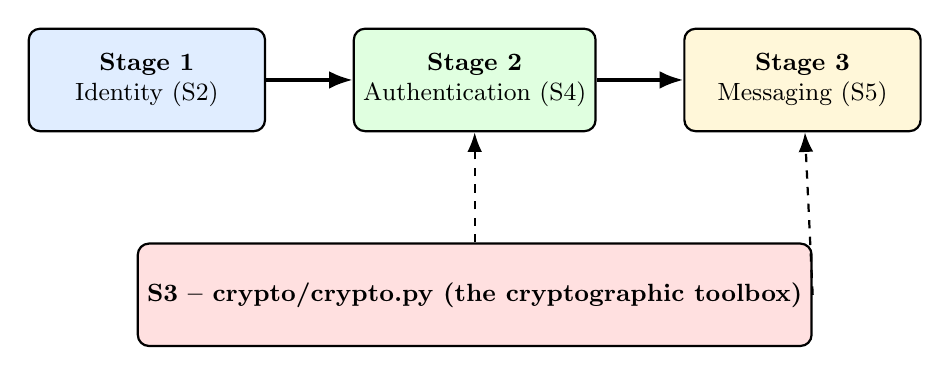
\begin{tikzpicture}[node distance=8mm and 11mm,every node/.style={font=\small},
    stage/.style={draw,rounded corners,minimum width=3.0cm,minimum height=1.3cm,
                  align=center,thick}]
  \node[stage,fill=boxblue]   (id)   {\textbf{Stage 1}\\Identity (S2)};
  \node[stage,fill=green!12,right=of id]   (auth) {\textbf{Stage 2}\\Authentication (S4)};
  \node[stage,fill=boxyellow,right=of auth] (msg) {\textbf{Stage 3}\\Messaging (S5)};
  \node[stage,fill=red!12,below=14mm of auth,minimum width=8.5cm] (core)
       {\textbf{S3 -- crypto/crypto.py (the cryptographic toolbox)}};
  \draw[-{Latex[length=3mm]},very thick] (id)   -- (auth);
  \draw[-{Latex[length=3mm]},very thick] (auth) -- (msg);
  \draw[-{Latex[length=2.5mm]},thick,dashed] (core) -- (auth);
  \draw[-{Latex[length=2.5mm]},thick,dashed] (core.east) -- (msg);
  \node[right=2mm of core.south east,font=\scriptsize\itshape] {};
\end{tikzpicture}
\end{center}

% =====================================================================
\section{The Theory You Must Study}
% =====================================================================

\subsection{Symmetric Encryption and AES}
\textbf{Plain definition.} \emph{Symmetric encryption} scrambles a message
(\emph{plaintext}) into unreadable \emph{ciphertext} using a secret key, and the
\emph{same} key unscrambles it. \textbf{AES} (Advanced Encryption Standard) is
the worldwide-standard symmetric cipher. ``AES-256'' means the key is 256 bits
(32 bytes) long.

\textbf{Real-life analogy.} A lockbox with one key. Whoever holds the key can
both lock things in and unlock them. The box without the key is just an opaque
brick --- you cannot see what is inside.

\textbf{Why it exists.} Symmetric encryption is \emph{fast} --- fast enough to
encrypt every safety message a car sends. (Public-key crypto, by contrast, is
slow; that is why it is used only for the handshake, not for every BSM.)

\textbf{How it works here.} The project uses AES with a 256-bit key
(\texttt{AES\_KEY\_LENGTH = 32}). The key itself comes from the handshake (S4).
The function \texttt{aes\_gcm\_encrypt} enforces the size: ``key must be exactly
32 bytes''.

\textbf{Security property it provides.} \textbf{Confidentiality}.

\subsection{Authenticated Encryption and AES-256-GCM}
\textbf{Plain definition.} \emph{Authenticated encryption} does two jobs in one
operation: it hides the message (confidentiality) \emph{and} produces a small
checksum-like value that detects any change (integrity). \textbf{GCM}
(Galois/Counter Mode) is the ``mode'' that adds the integrity job to AES.

\textbf{Real-life analogy.} Tamper-evident packaging on medicine. The box hides
the pills (confidentiality) \emph{and} carries a seal that visibly breaks if
anyone opened it (integrity). You get both protections from one package.

\textbf{Why it exists.} Plain encryption hides content but does \emph{not} stop
an attacker from flipping bits in the ciphertext. The receiver would happily
decrypt the corrupted message. GCM closes this hole by refusing to decrypt if
the message was changed.

\textbf{How it works here.} \texttt{aes\_gcm\_encrypt} returns three things:
\begin{itemize}
  \item the \textbf{ciphertext} --- the scrambled message;
  \item the \textbf{nonce} --- a 12-byte one-time value;
  \item the \textbf{authentication tag} --- a 16-byte (128-bit) ``seal''
        computed over the whole ciphertext.
\end{itemize}
On decryption, GCM recomputes the tag and compares. If even one bit changed, the
tags differ and the library raises \texttt{InvalidTag} --- the code turns this
into a \texttt{DecryptionError}.

\textbf{Security property it provides.} \textbf{Confidentiality} and
\textbf{integrity} together. AES-256-GCM is the same authenticated cipher used
by TLS~1.3.

\subsection{The Nonce}
\textbf{Plain definition.} A \emph{nonce} (``number used once'') is a value used
exactly once with a given key. AES-GCM needs a fresh 12-byte nonce for every
single encryption.

\textbf{Real-life analogy.} A single-use serial number on every parcel. Two
parcels must never carry the same number.

\textbf{Why it exists.} If you encrypt two different messages with the \emph{same}
key \emph{and} the same nonce, AES-GCM's security collapses --- an attacker can
learn relationships between the messages and even forge the tag. The nonce makes
each encryption unique.

\textbf{How it works here.} \texttt{aes\_gcm\_encrypt} calls
\texttt{os.urandom(12)} --- 12 cryptographically random bytes --- for every
message. With 96 random bits the chance of an accidental repeat is negligible.
The nonce is \emph{not} secret; it is sent alongside the ciphertext because the
receiver needs it to decrypt.

\textbf{Security property it provides.} It \emph{protects} confidentiality and
integrity by keeping every encryption unique.

\subsection{ECDH --- Elliptic-Curve Diffie--Hellman Key Exchange}
\textbf{Plain definition.} ECDH is a method by which two parties, each with their
own key pair, can compute the \emph{same} shared secret number --- and an
eavesdropper who sees both public keys still cannot compute it.

\textbf{Real-life analogy (the paint analogy).} Alice and Bob each start with a
secret paint colour. They mix their secret into a public colour and swap the
mixtures in the open. Each then mixes their own secret into the mixture they
received. Both end up with the identical final colour --- yet an eavesdropper who
saw only the swapped mixtures cannot un-mix them to find it.

\textbf{Why it exists.} It solves the key-distribution problem: two cars that
have never met can agree on a secret AES key over a channel the attacker is
watching, \emph{without ever transmitting the key}.

\textbf{How it works here (the mathematics, gently).} On the P-256 curve there is
a fixed public point $G$. A private key is a secret number $a$; the matching
public key is the point $a\cdot G$ (computed by ``hopping'' $G$ along the curve
$a$ times). The shared-secret magic is:
\[
a\cdot(b\cdot G)\;=\;ab\cdot G\;=\;b\cdot(a\cdot G).
\]
Vehicle~A computes $a\cdot(B\text{'s public})$; Vehicle~B computes
$b\cdot(A\text{'s public})$; both get $ab\cdot G$. An attacker sees $a\cdot G$
and $b\cdot G$ but cannot recover $a$ or $b$ (the ``elliptic-curve discrete
logarithm problem'' is infeasible). In code this is one line:
\texttt{my\_private\_key.exchange(ec.ECDH(), peer\_public\_key)}.

\textbf{Security property it provides.} It is the basis of
\textbf{confidentiality} and, because the project uses \emph{fresh} ECDH keys
each session, of \textbf{forward secrecy}.

\subsection{Ephemeral Keys and Forward Secrecy}
\textbf{Plain definition.} An \emph{ephemeral} key is generated fresh for one
session and thrown away afterwards. \textbf{Forward secrecy} is the guarantee
that recording today's encrypted traffic and stealing a key \emph{tomorrow} does
not let the attacker decrypt today's traffic.

\textbf{Real-life analogy.} A self-destructing one-time code. Even if someone
later finds your code notebook, today's code is already gone, so today's messages
stay locked forever.

\textbf{How it works here.} \texttt{generate\_ecdh\_keypair} creates a brand-new
P-256 key pair every time it is called, and the handshake calls it once per
session. The comment in the code says it plainly: ``even if an old key leaks
later, past sessions can't be decrypted because this key no longer exists.''

\textbf{Security property it provides.} \textbf{Forward secrecy}.

\subsection{HKDF --- Turning a Raw Secret into a Real Key}
\textbf{Plain definition.} HKDF (HMAC-based Key Derivation Function) is a
function that takes a rough, possibly non-uniform secret and produces a clean,
fixed-length, uniformly random key.

\textbf{Real-life analogy.} The raw ECDH output is like muddy river water ---
there is good water in it, but it is not fit to drink as-is. HKDF is the
filtration plant: in goes the rough secret, out comes clean, drinkable,
standard-sized water (a 32-byte AES key).

\textbf{Why it exists.} The raw number ECDH produces is secret, but its bits are
\emph{not} perfectly uniform, and you often want a key of an exact size. Feeding
the raw secret straight into AES is poor practice. HKDF fixes both issues. It
also lets you mix in extra public data so the final key is unique to this
session.

\textbf{How it works here.} \texttt{derive\_session\_key} calls HKDF with:
\begin{itemize}
  \item \texttt{algorithm = SHA256} --- the hash HKDF is built on;
  \item \texttt{length = 32} --- produce exactly a 32-byte AES-256 key;
  \item \texttt{salt = nonce\_a + nonce\_b} --- the two handshake nonces joined,
        making the key unique to this session;
  \item \texttt{info = b"v2v-session-key-v1"} --- a label tying the key to this
        exact purpose.
\end{itemize}
The same raw secret plus the same two nonces always yields the same 32-byte key
--- which is why both vehicles end up with an identical session key.

\textbf{Security property it provides.} It strengthens \textbf{confidentiality}
by producing a sound key, and ties the key to this session.

\subsection{SHA-256 Hashing}
\textbf{Plain definition.} A hash function turns any input into a short,
fixed-size fingerprint (SHA-256 $\to$ 256 bits). Same input, same fingerprint;
any change, completely different fingerprint; you cannot run it backwards.

\textbf{Why it exists here.} Two of S3's tools rely on it: HKDF is built on
SHA-256, and ECDSA signs the SHA-256 hash of the message rather than the whole
message.

\textbf{Security property it provides.} Supports \textbf{integrity}.

\subsection{ECDSA --- Digital Signatures}
\textbf{Plain definition.} ECDSA produces a signature with a \emph{private} key
that anyone with the matching \emph{public} key can verify. It proves \emph{who}
created the message and that it has \emph{not changed}.

\textbf{Real-life analogy.} A handwritten signature that is impossible to forge
and that also changes if the document is edited --- so the signature both
identifies the author and protects the text.

\textbf{Why it exists.} Encryption hides a message but does not prove who sent
it. A signature proves authorship, so the sender cannot later deny it.

\textbf{How it works here.} \texttt{ecdsa\_sign} calls
\texttt{private\_key.sign(message, ec.ECDSA(SHA256()))}; \texttt{ecdsa\_verify}
calls \texttt{public\_key.verify(signature, message, ec.ECDSA(SHA256()))}. The
signature is returned in \textbf{DER} encoding --- a compact standard binary
format.

\textbf{Security property it provides.} \textbf{Authentication},
\textbf{integrity}, \textbf{non-repudiation}.

\subsection{PEM Serialization of Keys}
\textbf{Plain definition.} \emph{Serialization} means turning a key object in
memory into bytes that can be saved or sent; \emph{loading} is the reverse. PEM
is the text format (Base64 between BEGIN/END lines) used.

\textbf{Why it exists here.} During the handshake a vehicle must \emph{send} its
ephemeral ECDH public key to the other vehicle. You cannot send a Python object
over a network --- you send bytes. \texttt{serialize\_public\_key} produces those
bytes; \texttt{load\_public\_key} rebuilds the key object on the other side.

\textbf{Security property it provides.} None directly --- it is about
\emph{format}. (A public key is meant to be shared, so there is nothing secret to
protect here.)

% =====================================================================
\section{Code Walkthrough}
% =====================================================================

\texttt{crypto/crypto.py} is organised as: three custom exceptions, a tiny
type-checking helper, then the four tool groups (AES-GCM, ECDH+HKDF, ECDSA, PEM),
then a built-in demonstration.

\subsection{The custom exceptions and the type guard}
\begin{lstlisting}[style=py,caption={crypto.py --- custom exceptions and the bytes guard.}]
class CryptoError(Exception):
    """Base exception for cryptographic errors in this simulation."""

class DecryptionError(CryptoError):
    """Raised when AES-GCM authentication fails during decryption."""

class SignatureError(CryptoError):
    """Raised when signature-related operations fail."""

def _ensure_bytes(value: bytes, name: str) -> None:
    if not isinstance(value, bytes):
        raise TypeError(f"{name} must be bytes")
\end{lstlisting}
\textbf{Explanation:}
\begin{enumerate}
  \item \texttt{CryptoError} is the \emph{parent} of all crypto errors, so other
        code can catch every crypto problem with one \texttt{except}.
  \item \texttt{DecryptionError} specifically means ``the message failed its
        integrity check'' --- i.e.\ possible tampering.
  \item \texttt{SignatureError} means a signing operation failed.
  \item \texttt{\_ensure\_bytes} is a small helper: cryptographic functions must
        be given raw \texttt{bytes}, not text strings. The leading underscore is
        a Python convention meaning ``private --- internal use only''.
\end{enumerate}

\subsection{aes\_gcm\_encrypt() --- lock a message}
\textbf{Purpose:} encrypt a message with AES-256-GCM, returning ciphertext, nonce
and tag.
\begin{lstlisting}[style=py,caption={crypto.py --- AES-256-GCM encryption.}]
def aes_gcm_encrypt(key: bytes, plaintext: bytes) -> tuple[bytes, bytes, bytes]:
    _ensure_bytes(key, "key")
    _ensure_bytes(plaintext, "plaintext")

    if len(key) != 32:
        raise ValueError("key must be exactly 32 bytes for AES-256-GCM")

    nonce = os.urandom(12)
    aesgcm = AESGCM(key)
    encrypted_blob = aesgcm.encrypt(nonce, plaintext, None)
    ciphertext = encrypted_blob[:-16]
    auth_tag = encrypted_blob[-16:]
    return ciphertext, nonce, auth_tag
\end{lstlisting}
\textbf{Step by step:}
\begin{enumerate}
  \item Check both arguments are \texttt{bytes}.
  \item Check the key is exactly 32 bytes --- that is what makes it AES-\emph{256}.
        A wrong size raises \texttt{ValueError}.
  \item \texttt{os.urandom(12)} draws a fresh 12-byte random nonce --- new for
        every call.
  \item \texttt{AESGCM(key)} creates the cipher object bound to that key.
  \item \texttt{aesgcm.encrypt(nonce, plaintext, None)} encrypts. The third
        argument is the \emph{associated data} (extra data to authenticate but
        not encrypt); \texttt{None} means none is used here. The library returns
        a single blob: \texttt{ciphertext} followed by the 16-byte tag.
  \item \texttt{encrypted\_blob[:-16]} is everything except the last 16 bytes ---
        the ciphertext. \texttt{encrypted\_blob[-16:]} is the last 16 bytes ---
        the authentication tag. The code splits them so callers can store them
        separately.
\end{enumerate}
\textbf{Arguments:} \texttt{key} (32 bytes), \texttt{plaintext} (bytes).
\textbf{Returns:} a 3-tuple \texttt{(ciphertext, nonce, auth\_tag)}.
\textbf{Exceptions:} \texttt{TypeError} (not bytes), \texttt{ValueError} (key not
32 bytes). \textbf{Theory link:} authenticated encryption, the nonce, the tag.
\emph{Analogy:} sealing the message in tamper-evident packaging and printing a
fresh serial number (nonce) on it.

\subsection{aes\_gcm\_decrypt() --- unlock and verify}
\textbf{Purpose:} decrypt AES-GCM ciphertext \emph{and} verify it was not
tampered with.
\begin{lstlisting}[style=py,caption={crypto.py --- AES-256-GCM decryption with tamper detection.}]
def aes_gcm_decrypt(key, ciphertext, nonce, tag) -> bytes:
    _ensure_bytes(key, "key"); _ensure_bytes(ciphertext, "ciphertext")
    _ensure_bytes(nonce, "nonce"); _ensure_bytes(tag, "tag")

    if len(key) != 32:   raise ValueError("key must be exactly 32 bytes ...")
    if len(nonce) != 12: raise ValueError("nonce must be exactly 12 bytes ...")
    if len(tag) != 16:   raise ValueError("tag must be exactly 16 bytes ...")

    encrypted_blob = ciphertext + tag
    aesgcm = AESGCM(key)
    try:
        return aesgcm.decrypt(nonce, encrypted_blob, None)
    except InvalidTag as exc:
        raise DecryptionError(
            "Message authentication failed - possible tampering detected"
        ) from exc
\end{lstlisting}
\textbf{Step by step:}
\begin{enumerate}
  \item Check all four arguments are \texttt{bytes}.
  \item Check the exact lengths: key 32, nonce 12, tag 16. Any wrong size raises
        \texttt{ValueError} --- a clear ``programmer error'' rather than a
        security event.
  \item Re-join \texttt{ciphertext + tag} into the single blob the library
        expects (the opposite of the split done during encryption).
  \item \texttt{aesgcm.decrypt(...)} does two things in one step: it decrypts and
        it re-computes the tag and compares it.
  \item If the tag matches, it returns the original plaintext. If the ciphertext,
        nonce or tag was altered, the library raises \texttt{InvalidTag}; the
        code catches it and re-raises a friendlier \texttt{DecryptionError}.
\end{enumerate}
\textbf{The crucial idea:} a tampered message does \emph{not} decrypt to garbage
--- it \emph{refuses to decrypt at all}. There is no way to ``ignore'' a bad tag.
\textbf{Theory link:} authenticated encryption providing integrity.
\emph{Analogy:} the pharmacist seeing the broken seal and refusing to hand over
the medicine.

\subsection{generate\_ecdh\_keypair() --- a fresh key pair per session}
\begin{lstlisting}[style=py,caption={crypto.py --- generate an ephemeral ECDH key pair.}]
def generate_ecdh_keypair():
    # We generate a NEW key pair each session (ephemeral).
    # This provides "Forward Secrecy".
    private_key = ec.generate_private_key(ec.SECP256R1(), default_backend())
    public_key = private_key.public_key()
    return private_key, public_key
\end{lstlisting}
\textbf{Step by step:} create a new P-256 private key; derive its public key;
return both. There are no arguments. \textbf{Returns:} a tuple
\texttt{(private\_key, public\_key)}. \textbf{Theory link:} ephemeral keys and
forward secrecy --- because it is called fresh for each session, an old key
simply does not exist any more.

\subsection{ecdh\_shared\_secret() --- compute the shared number}
\begin{lstlisting}[style=py,caption={crypto.py --- ECDH shared-secret computation.}]
def ecdh_shared_secret(my_private_key, peer_public_key) -> bytes:
    if not isinstance(my_private_key, ec.EllipticCurvePrivateKey):
        raise TypeError("my_private_key must be an EllipticCurvePrivateKey")
    if not isinstance(peer_public_key, ec.EllipticCurvePublicKey):
        raise TypeError("peer_public_key must be an EllipticCurvePublicKey")
    try:
        return my_private_key.exchange(ec.ECDH(), peer_public_key)
    except Exception as exc:
        raise CryptoError("failed to compute ECDH shared secret") from exc
\end{lstlisting}
\textbf{Step by step:}
\begin{enumerate}
  \item Confirm the first argument is a private key and the second is a public key.
  \item \texttt{my\_private\_key.exchange(ec.ECDH(), peer\_public\_key)} performs
        the elliptic-curve multiplication $a\cdot(b\cdot G)$ and returns the raw
        shared-secret bytes.
  \item Any failure is wrapped as a \texttt{CryptoError}.
\end{enumerate}
\textbf{Key fact:} if Vehicle~A calls this with (A-private, B-public) and
Vehicle~B calls it with (B-private, A-public), \emph{both get the identical
bytes}. \textbf{Returns:} the raw shared secret (bytes). \textbf{Theory link:}
ECDH key exchange. \emph{Analogy:} both painters finishing with the same final
colour.

\subsection{derive\_session\_key() --- raw secret to clean AES key}
\begin{lstlisting}[style=py,caption={crypto.py --- HKDF key derivation.}]
def derive_session_key(shared_secret, nonce_a, nonce_b) -> bytes:
    _ensure_bytes(shared_secret, "shared_secret")
    _ensure_bytes(nonce_a, "nonce_a")
    _ensure_bytes(nonce_b, "nonce_b")

    hkdf = HKDF(
        algorithm=hashes.SHA256(),
        length=32,
        salt=nonce_a + nonce_b,
        info=b"v2v-session-key-v1",
        backend=default_backend(),
    )
    return hkdf.derive(shared_secret)
\end{lstlisting}
\textbf{Step by step:}
\begin{enumerate}
  \item Check all three arguments are bytes.
  \item Build an \texttt{HKDF} object: SHA-256 as the base hash;
        \texttt{length=32} so the output is exactly an AES-256 key;
        \texttt{salt} is the two session nonces joined together;
        \texttt{info} is the fixed purpose label.
  \item \texttt{hkdf.derive(shared\_secret)} runs the raw ECDH secret through
        HKDF and returns the clean 32-byte key.
\end{enumerate}
\textbf{Why salt = nonce\_a + nonce\_b?} The raw ECDH secret could repeat if the
same ephemeral keys were ever reused; mixing in two fresh random nonces
guarantees the \emph{derived} key is unique to this session.
\textbf{Honest note:} the string \texttt{b"v2v-session-key-v1"} is written
directly here even though \texttt{config.py} already defines
\texttt{SESSION\_KEY\_INFO} with the same value --- a small duplication worth
mentioning if asked. \textbf{Returns:} a 32-byte key. \textbf{Theory link:} HKDF.
\emph{Analogy:} the filtration plant turning muddy water into clean water.

\subsection{ecdsa\_sign() and ecdsa\_verify() --- digital signatures}
\begin{lstlisting}[style=py,caption={crypto.py --- ECDSA signing and verification.}]
def ecdsa_sign(private_key, message: bytes) -> bytes:
    if not isinstance(private_key, ec.EllipticCurvePrivateKey):
        raise TypeError("private_key must be an EllipticCurvePrivateKey")
    _ensure_bytes(message, "message")
    try:
        return private_key.sign(message, ec.ECDSA(hashes.SHA256()))
    except Exception as exc:
        raise SignatureError("failed to create ECDSA signature") from exc

def ecdsa_verify(public_key, message: bytes, signature: bytes) -> bool:
    if not isinstance(public_key, ec.EllipticCurvePublicKey):
        raise TypeError("public_key must be an EllipticCurvePublicKey")
    _ensure_bytes(message, "message")
    _ensure_bytes(signature, "signature")
    try:
        public_key.verify(signature, message, ec.ECDSA(hashes.SHA256()))
        return True
    except InvalidSignature:
        return False
\end{lstlisting}
\textbf{ecdsa\_sign --- step by step:}
\begin{enumerate}
  \item Confirm the key is a private key and the message is bytes.
  \item \texttt{private\_key.sign(message, ec.ECDSA(SHA256()))} hashes the
        message with SHA-256 and signs that hash. It returns the signature in
        DER encoding.
  \item Any failure becomes a \texttt{SignatureError}.
\end{enumerate}
\textbf{ecdsa\_verify --- step by step:}
\begin{enumerate}
  \item Confirm the key is a public key and the other two arguments are bytes.
  \item \texttt{public\_key.verify(signature, message, ec.ECDSA(SHA256()))}
        re-hashes the message and checks the signature against it.
  \item If valid, \texttt{verify} returns silently and the function returns
        \texttt{True}. If invalid it raises \texttt{InvalidSignature}, which is
        caught and turned into \texttt{False}.
\end{enumerate}
\textbf{Design note:} \texttt{ecdsa\_verify} returns a plain
\texttt{True}/\texttt{False} rather than raising --- this makes it easy for the
handshake code to write \texttt{if not ecdsa\_verify(...)}. \textbf{Theory link:}
ECDSA, authentication, integrity, non-repudiation. \emph{Analogy:} pressing the
wax seal (sign) and inspecting it (verify).

\subsection{serialize\_public\_key(), load\_public\_key(), load\_private\_key()}
These three are the PEM bridge between in-memory key objects and bytes.
\begin{lstlisting}[style=py,caption={crypto.py --- PEM serialization helpers.}]
def serialize_public_key(pub_key) -> bytes:
    if not isinstance(pub_key, ec.EllipticCurvePublicKey):
        raise TypeError("pub_key must be an EllipticCurvePublicKey")
    return pub_key.public_bytes(
        encoding=serialization.Encoding.PEM,
        format=serialization.PublicFormat.SubjectPublicKeyInfo,
    )

def load_public_key(pem_data: bytes) -> ec.EllipticCurvePublicKey:
    _ensure_bytes(pem_data, "pem_data")
    try:
        public_key = serialization.load_pem_public_key(pem_data, backend=default_backend())
    except Exception as exc:
        raise ValueError("invalid PEM public key data") from exc
    if not isinstance(public_key, ec.EllipticCurvePublicKey):
        raise ValueError("loaded key is not an elliptic-curve public key")
    return public_key
\end{lstlisting}
\textbf{Explanation:}
\begin{enumerate}
  \item \texttt{serialize\_public\_key} turns a public-key object into PEM text
        bytes (so it can be put inside a handshake message and sent).
  \item \texttt{load\_public\_key} parses PEM bytes back into a key object, and
        rejects anything that is not a valid elliptic-curve public key.
  \item \texttt{load\_private\_key} (not shown, same shape) parses a PEM private
        key with \texttt{password=None}, matching the un-encrypted key files from
        S2.
\end{enumerate}
\textbf{Theory link:} PEM serialization. \emph{Analogy:} flattening a 3-D object
into a printed sheet so it can be posted, then folding it back up on arrival.

\subsection{The built-in demonstration (\texttt{if \_\_name\_\_ == "\_\_main\_\_"})}
At the bottom of the file is a five-test self-demonstration that runs only when
the file is executed directly. It is excellent for learning because it exercises
every tool: Test~1 proves ECDH gives both sides the same secret; Test~2 derives a
session key; Test~3 encrypts then decrypts a message; Test~4 signs and verifies
(and shows verification \emph{fails} with the wrong key); Test~5 flips one bit of
ciphertext and confirms the tampered message is rejected. We run it in the next
section.

% =====================================================================
\section{Hands-On / Practical}
% =====================================================================

\subsection{Run the cryptographic core by itself}
\texttt{crypto.py} needs no certificates and no network --- just run it:
\begin{lstlisting}[style=term]
python crypto\crypto.py
\end{lstlisting}

\noindent\textbf{Expected output (sample). Note: where this guide shows
\texttt{[OK]}, the real terminal prints a small check-mark character, because the
source uses the escape \texttt{\textbackslash u2713}.}
\begin{lstlisting}[style=term]
=== CRYPTO MODULE DEMONSTRATION ===

[TEST 1] ECDH Key Exchange
Vehicle A secret == Vehicle B secret: True

[TEST 2] Session Key Derivation
Session key (hex): 9f3c1a...e7b2   (64 hex characters)
Session key length: 32 bytes

[TEST 3] AES-GCM Encrypt/Decrypt
Decrypted: Hello from Vehicle A! [OK]

[TEST 4] ECDSA Sign/Verify
Signature valid with matching key: True
Signature valid with wrong key: False

[TEST 5] Tamper Detection
Tampered message correctly rejected [OK]
\end{lstlisting}

\subsection{What each output line means}
\begin{itemize}
  \item \textbf{Test 1 --- \texttt{True}}: the two vehicles, using only each
        other's \emph{public} keys, computed the \emph{same} secret. ECDH works.
  \item \textbf{Test 2 --- 32 bytes}: HKDF turned the raw secret into exactly a
        256-bit AES key. The hex string is 64 characters because each byte is two
        hex digits.
  \item \textbf{Test 3 --- ``Decrypted: Hello from Vehicle A!''}: encrypt then
        decrypt round-trips perfectly --- confidentiality with no data loss.
  \item \textbf{Test 4 --- \texttt{True} then \texttt{False}}: the signature
        verifies with the correct public key, but \emph{fails} with the wrong
        key. That ``False'' is exactly how impersonation is detected.
  \item \textbf{Test 5 --- ``rejected''}: one bit of ciphertext was flipped;
        decryption refused. That is the tamper defence working.
\end{itemize}

\subsection{Try This Yourself (mini-experiment): break the tag}
Test~5 already flips a \emph{ciphertext} bit. Try flipping the \emph{tag}
instead. Add a few lines to the demo (or open a Python shell):
\begin{lstlisting}[style=term]
ct, nc, tag = aes_gcm_encrypt(session_key, b"hello")
bad_tag = bytearray(tag)
bad_tag[0] ^= 0x01                       # flip one bit of the tag
aes_gcm_decrypt(session_key, ct, nc, bytes(bad_tag))
\end{lstlisting}
\textbf{Predict before you run.} The tag is part of what GCM checks, so a changed
tag is just as fatal as changed ciphertext. Prediction: a
\texttt{DecryptionError} (``possible tampering detected'') is raised. Lesson: the
nonce, the ciphertext \emph{and} the tag are all protected --- you cannot edit
any of them and still decrypt.

\textbf{Second experiment:} keep the ciphertext and tag correct but change the
\emph{nonce} by one bit. Predict: still a \texttt{DecryptionError}, because the
tag was computed for the original nonce.

% =====================================================================
\section{Attack Relevance}
% =====================================================================

S3 is the \emph{toolbox}, so it supplies the defence used against \emph{three}
of the four attacks. The defences are exercised directly by
\texttt{attacks/tamper\_attack.py}.

\begin{table}[h]
\centering
\small
\begin{tabular}{@{}p{2.6cm} p{6.0cm} p{4.9cm}@{}}
\toprule
\textbf{Attack} & \textbf{How an S3 tool stops it} & \textbf{The function}\\
\midrule
Tamper & Any change to ciphertext, nonce or tag makes the GCM tag mismatch;
decryption refuses. & \texttt{aes\_gcm\_decrypt} (raises \texttt{DecryptionError}).\\
Eavesdrop & The message is AES-256 ciphertext; without the session key it is
unreadable noise. & \texttt{aes\_gcm\_encrypt}.\\
Impersonation & A forged message will not carry a signature that verifies under
the real vehicle's public key. & \texttt{ecdsa\_verify} (returns \texttt{False}).\\
\bottomrule
\end{tabular}
\caption{Which S3 tool defends against which attack.}
\end{table}

\noindent\textbf{The tamper attack in detail.} The attacker captures an encrypted
BSM and flips bits hoping to change ``speed 80'' into something dangerous. But
the AES-GCM tag is computed over the \emph{whole} ciphertext. The receiver's call
to \texttt{aes\_gcm\_decrypt} re-computes the tag, sees a mismatch, and raises
\texttt{DecryptionError} instead of returning data. The attacker cannot fix the
tag because they do not have the session key. \textbf{Forward secrecy} is also an
S3 contribution: \texttt{generate\_ecdh\_keypair} makes a throw-away key each
session, so a key stolen later cannot decrypt recorded traffic.

\textbf{Honest scope note.} S3 provides the \emph{primitives}; it does not by
itself decide \emph{when} to use them or check timestamps and nonces --- that
sequencing is the protocol logic in S4 and S5. A primitive used incorrectly (for
example, reusing a nonce) would still be insecure; S3 just makes correct use
possible.

% =====================================================================
\section{Illustrations}
% =====================================================================

\subsection{Diagram 1 --- AES-256-GCM Encrypt then Decrypt}
\begin{center}
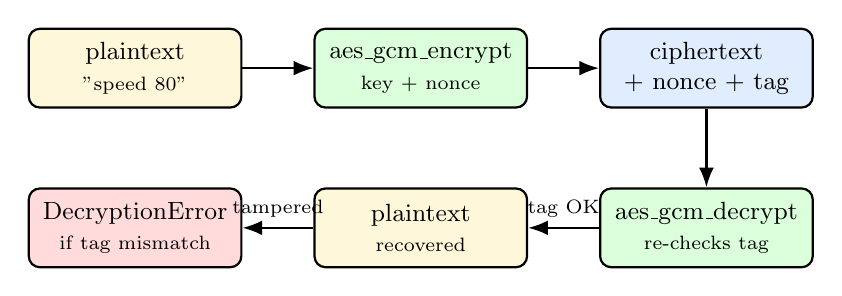
\begin{tikzpicture}[font=\small,node distance=6mm,
   box/.style={draw,thick,rounded corners,minimum width=2.7cm,minimum height=1.0cm,
               align=center}]
  \node[box,fill=boxyellow] (pt) {plaintext\\\scriptsize "speed 80"};
  \node[box,fill=green!14,right=9mm of pt] (enc) {aes\_gcm\_encrypt\\\scriptsize key + nonce};
  \node[box,fill=boxblue,right=9mm of enc] (out) {ciphertext\\+ nonce + tag};
  \node[box,fill=green!14,below=10mm of out] (dec) {aes\_gcm\_decrypt\\\scriptsize re-checks tag};
  \node[box,fill=boxyellow,left=9mm of dec] (pt2) {plaintext\\\scriptsize recovered};
  \node[box,fill=red!14,left=9mm of pt2] (fail) {DecryptionError\\\scriptsize if tag mismatch};
  \draw[-{Latex[length=2.5mm]},thick] (pt) -- (enc);
  \draw[-{Latex[length=2.5mm]},thick] (enc) -- (out);
  \draw[-{Latex[length=2.5mm]},thick] (out) -- (dec);
  \draw[-{Latex[length=2.5mm]},thick] (dec) -- (pt2) node[midway,above,font=\scriptsize]{tag OK};
  \draw[-{Latex[length=2.5mm]},thick] (pt2) -- (fail) node[midway,above,font=\scriptsize]{tampered};
\end{tikzpicture}
\end{center}

\subsection{Diagram 2 --- ECDH gives both sides the same secret}
\begin{center}
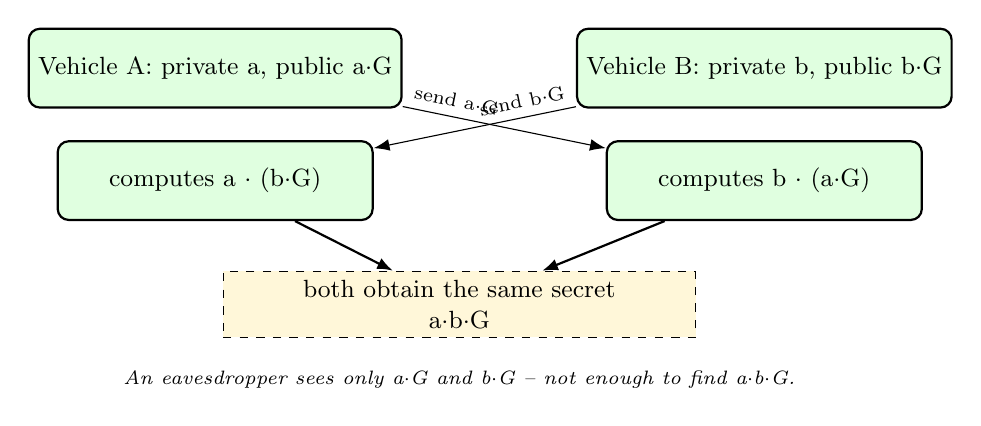
\begin{tikzpicture}[font=\small,node distance=5mm,
   v/.style={draw,thick,rounded corners,fill=green!12,minimum width=4.0cm,
             minimum height=1.0cm,align=center}]
  \node[v] (a1) {Vehicle A: private a, public a$\cdot$G};
  \node[v,below=4mm of a1] (a2) {computes a $\cdot$ (b$\cdot$G)};
  \node[v,right=22mm of a1] (b1) {Vehicle B: private b, public b$\cdot$G};
  \node[v,below=4mm of b1] (b2) {computes b $\cdot$ (a$\cdot$G)};
  \node[draw,dashed,fill=boxyellow,minimum width=6cm,align=center] (s)
       at (3.1,-3.0)
       {both obtain the same secret\\ a$\cdot$b$\cdot$G};
  \draw[-{Latex[length=2mm]}] (a1) -- (b2)
       node[pos=0.25,above,font=\scriptsize,sloped]{send a$\cdot$G};
  \draw[-{Latex[length=2mm]}] (b1) -- (a2)
       node[pos=0.25,above,font=\scriptsize,sloped]{send b$\cdot$G};
  \draw[-{Latex[length=2mm]},thick] (a2) -- (s);
  \draw[-{Latex[length=2mm]},thick] (b2) -- (s);
  \node[below=3mm of s,font=\scriptsize\itshape]
       {An eavesdropper sees only a$\cdot$G and b$\cdot$G -- not enough to find a$\cdot$b$\cdot$G.};
\end{tikzpicture}
\end{center}

\subsection{Diagram 3 --- The S3 pipeline that builds a session key}
\begin{center}
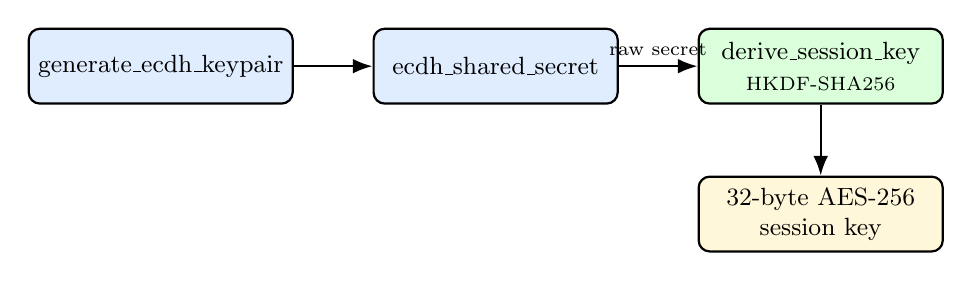
\begin{tikzpicture}[font=\small,node distance=8mm,
   box/.style={draw,thick,rounded corners,minimum width=3.1cm,minimum height=0.95cm,
               align=center}]
  \node[box,fill=boxblue] (kp) {generate\_ecdh\_keypair};
  \node[box,fill=boxblue,right=10mm of kp] (ss) {ecdh\_shared\_secret};
  \node[box,fill=green!14,right=10mm of ss] (dk) {derive\_session\_key\\\scriptsize HKDF-SHA256};
  \node[box,fill=boxyellow,below=9mm of dk] (key) {32-byte AES-256\\session key};
  \draw[-{Latex[length=2.5mm]},thick] (kp) -- (ss);
  \draw[-{Latex[length=2.5mm]},thick] (ss) -- (dk) node[midway,above,font=\scriptsize]{raw secret};
  \draw[-{Latex[length=2.5mm]},thick] (dk) -- (key);
\end{tikzpicture}
\end{center}

% =====================================================================
\section{Presentation Pack}
% =====================================================================

\subsection{Slide Outline}

\textbf{Slide 1 --- The Crypto Toolbox.}
\begin{itemize}
  \item \texttt{crypto.py} is a library, not a program --- four tools.
  \item AES-256-GCM: lock + tamper seal. ECDH: agree a secret. HKDF: clean the
        secret. ECDSA: sign.
  \item Every later section calls these functions.
  \item Industry-standard --- the same set used by TLS 1.3.
\end{itemize}

\textbf{Slide 2 --- AES-256-GCM: Authenticated Encryption.}
\begin{itemize}
  \item Encrypt returns three things: ciphertext, nonce, 16-byte tag.
  \item The tag is a seal over the whole ciphertext.
  \item Decrypt re-checks the tag; one changed bit $\to$ \texttt{DecryptionError}.
  \item Gives confidentiality AND integrity in one step.
\end{itemize}

\textbf{Slide 3 --- ECDH + HKDF: Building a Shared Key.}
\begin{itemize}
  \item ECDH: two cars compute the same secret without sending it.
  \item Maths: a$\cdot$(b$\cdot$G) = b$\cdot$(a$\cdot$G).
  \item Keys are ephemeral $\to$ forward secrecy.
  \item HKDF filters the raw secret into a clean 32-byte AES key.
\end{itemize}

\textbf{Slide 4 --- ECDSA: Digital Signatures.}
\begin{itemize}
  \item Sign with the private key, verify with the public key.
  \item Proves who wrote it (authentication) and that it is unchanged (integrity).
  \item \texttt{ecdsa\_verify} returns \texttt{True}/\texttt{False}.
  \item Wrong key $\to$ \texttt{False} $\to$ impersonation detected.
\end{itemize}

\textbf{Slide 5 --- Live Proof: the Five-Test Demo.}
\begin{itemize}
  \item Test 1: ECDH secrets match. Test 2: 32-byte key derived.
  \item Test 3: encrypt/decrypt round-trips.
  \item Test 4: signature good with right key, fails with wrong key.
  \item Test 5: a flipped bit is rejected --- the tamper defence.
\end{itemize}

\subsection{Speaker Talking Points (about 30--60 seconds each)}

\textbf{Slide 1.} ``This section is one file, crypto.py, and it is unusual ---
it contains no networking and no protocol. It is purely a toolbox of four
cryptographic tools. AES-256-GCM is our lockbox with a built-in tamper seal. ECDH
lets two cars secretly agree on a key. HKDF cleans that key up. And ECDSA is our
unforgeable signature. Everything else in the project --- the handshake, the
secure messaging --- just calls these functions. And these are not toy
algorithms: this is the exact same set of building blocks used by TLS 1.3, the
security behind every HTTPS website.''

\textbf{Slide 2.} ``AES-256-GCM is authenticated encryption. When you encrypt,
you get back three things: the ciphertext, a nonce, and a 16-byte authentication
tag. Think of the tag as a wax seal stamped over the whole ciphertext. When you
decrypt, the library does not just unscramble --- it recomputes the tag and
compares. If even one bit of the ciphertext, the nonce or the tag was changed,
the tags disagree and decryption is refused; our code raises a DecryptionError.
So with one operation we get confidentiality --- the content is hidden --- and
integrity --- any change is caught.''

\textbf{Slide 3.} ``How do two cars that have never met get a shared secret key
over a channel an attacker is watching? That is ECDH. Each car has a private
number and a public point. They swap public points in the open. Then each mixes
its own private number with the other's public point. Thanks to the curve maths
--- a times b-times-G equals b times a-times-G --- both arrive at the identical
secret, while an eavesdropper who saw only the public points cannot compute it.
And because we generate a fresh ECDH key for every session and throw it away, a
key stolen tomorrow cannot unlock today's traffic --- that is forward secrecy.
Finally HKDF takes that raw secret, which is not perfectly uniform, and filters
it into a clean 32-byte AES key.''

\textbf{Slide 4.} ``ECDSA is our digital signature. You sign with your private
key; anyone can verify with your public key. A signature proves two things at
once: who created the message, and that it has not been changed since. In the
code, ecdsa\_verify simply returns True or False. And here is the security point
--- if an impostor signs a message with the wrong key, verification returns
False. That single False is how we catch impersonation.''

\textbf{Slide 5.} ``The best part is that crypto.py proves itself. Run it
directly and it executes five tests. Test one shows the two ECDH secrets are
equal. Test two shows HKDF produced a 32-byte key. Test three encrypts and
decrypts a message and recovers it exactly. Test four signs a message and shows
verification succeeds with the right key and fails with the wrong one. And test
five flips a single bit of ciphertext and shows the message is rejected. Five
tests, every tool, all visible on screen.''

\subsection{Live-Demo Script}
\begin{enumerate}
  \item \textbf{Run the toolbox.} Execute \texttt{python crypto\textbackslash
        crypto.py}. Point at \texttt{[TEST 1] ... True} --- ``both cars derived
        the same secret without sending it.''
  \item \textbf{Point at Test 2.} ``32 bytes --- that is our AES-256 key.''
  \item \textbf{Point at Test 4.} ``True with the right key, False with the
        wrong key --- that False is impersonation being caught.''
  \item \textbf{Point at Test 5.} ``One bit flipped, message rejected --- the
        tamper defence.''
  \item \textbf{Optional.} In a Python shell, flip a bit of the \emph{tag} (see
        the mini-experiment) and show the same \texttt{DecryptionError}.
\end{enumerate}

\subsection{Examiner Q\&A}
\begin{enumerate}
  \item \textbf{Q: What does the ``GCM'' in AES-256-GCM add over plain AES?}\\
        A: GCM (Galois/Counter Mode) adds \emph{authentication}: a 16-byte tag
        computed over the ciphertext. It turns AES into \emph{authenticated}
        encryption, giving integrity as well as confidentiality.
  \item \textbf{Q: Why must the nonce never repeat for the same key?}\\
        A: Reusing a (key, nonce) pair in GCM breaks security --- it can leak
        relationships between messages and allow tag forgery. The code uses a
        fresh \texttt{os.urandom(12)} nonce every time to prevent this.
  \item \textbf{Q: Is the nonce secret?}\\
        A: No. It is sent alongside the ciphertext because the receiver needs it
        to decrypt. Security depends on \emph{uniqueness}, not secrecy.
  \item \textbf{Q: How does ECDH let two cars share a key without sending it?}\\
        A: Each car combines its own private key with the other's public key.
        The curve maths makes both results equal (\,a$\cdot$b$\cdot$G\,), and an
        eavesdropper with only the public keys cannot compute it.
  \item \textbf{Q: Why use HKDF instead of using the ECDH output directly?}\\
        A: The raw ECDH secret is not perfectly uniform and may not be the right
        size. HKDF extracts and expands it into a clean, fixed-length key, and
        the nonce salt ties the key to this one session.
  \item \textbf{Q: What happens in \texttt{aes\_gcm\_decrypt} if a message is
        tampered with?}\\
        A: The recomputed tag does not match, the library raises
        \texttt{InvalidTag}, and the code re-raises it as \texttt{DecryptionError}
        --- no plaintext is ever returned.
  \item \textbf{Q: Why does \texttt{ecdsa\_verify} return a boolean instead of
        raising?}\\
        A: A failed signature is an expected, normal event during an attack, not
        a programming bug. Returning \texttt{False} lets callers write a simple
        \texttt{if not ecdsa\_verify(...)} check.
  \item \textbf{Q: This file is called a ``toolbox'' --- what does it \emph{not}
        do?}\\
        A: It provides primitives only. It does not check timestamps, manage
        nonces against replay, or sequence the handshake --- that protocol logic
        lives in S4 and S5. Correct \emph{use} of the primitives is the
        protocol's responsibility.
\end{enumerate}

% =====================================================================
\section{Glossary}
% =====================================================================
\begin{description}[style=nextline,leftmargin=0pt]
  \item[Plaintext] The original readable message before encryption.
  \item[Ciphertext] The scrambled, unreadable output of encryption.
  \item[Symmetric encryption] Encryption using one shared secret key for both directions.
  \item[AES] Advanced Encryption Standard: the worldwide-standard symmetric cipher.
  \item[AES-256] AES with a 256-bit (32-byte) key.
  \item[GCM] Galois/Counter Mode: the AES mode that adds an authentication tag.
  \item[Authenticated encryption] Encryption that also detects any tampering.
  \item[Nonce] A number used exactly once with a given key.
  \item[Authentication tag] The 16-byte value GCM computes to detect tampering.
  \item[Associated data (AAD)] Extra data authenticated but not encrypted (here: none).
  \item[ECDH] Elliptic-Curve Diffie--Hellman: a shared-secret key-exchange method.
  \item[Shared secret] The identical secret value two parties compute via ECDH.
  \item[Ephemeral key] A key generated for one session and then discarded.
  \item[Forward secrecy] Past traffic stays secret even if a key leaks later.
  \item[HKDF] HMAC-based Key Derivation Function: turns a raw secret into a clean key.
  \item[Salt] Extra input to HKDF (here the two nonces) making the key session-unique.
  \item[Info string] A label fed to HKDF binding the key to a specific purpose.
  \item[SHA-256] A hash function producing a 256-bit fingerprint.
  \item[ECDSA] Elliptic Curve Digital Signature Algorithm.
  \item[Digital signature] A private-key-made value verifiable with the public key.
  \item[DER] A compact binary encoding (used here for signatures).
  \item[PEM] A text encoding (Base64 + BEGIN/END lines) used for keys.
  \item[Serialization] Converting an in-memory object into bytes for storage/transmission.
  \item[InvalidTag] The library error raised when a GCM tag does not match.
  \item[DecryptionError] This project's exception meaning ``possible tampering''.
  \item[Session key] The 32-byte AES key used to encrypt one conversation.
\end{description}

% =====================================================================
\section{References and Further Study}
% =====================================================================
\begin{itemize}
  \item \textbf{Python cryptography --- AES-GCM (AESGCM) docs} ---
        \url{https://cryptography.io/en/latest/hazmat/primitives/aead/}\\
        Read for: the exact \texttt{AESGCM} class used in \texttt{crypto.py}.
  \item \textbf{Python cryptography --- elliptic-curve docs} ---
        \url{https://cryptography.io/en/latest/hazmat/primitives/asymmetric/ec/}\\
        Read for: ECDH \texttt{exchange()} and ECDSA \texttt{sign/verify}.
  \item \textbf{Python cryptography --- HKDF docs} ---
        \url{https://cryptography.io/en/latest/hazmat/primitives/key-derivation-functions/}\\
        Read for: the \texttt{HKDF} class, its salt and info parameters.
  \item \textbf{NIST SP 800-38D --- GCM mode of operation} ---
        \url{https://csrc.nist.gov/pubs/sp/800/38/d/final}\\
        Read for: the official definition of AES-GCM and the nonce rule.
  \item \textbf{NIST FIPS 197 --- the AES standard} ---
        \url{https://csrc.nist.gov/pubs/fips/197/final}\\
        Read for: what AES itself is.
  \item \textbf{RFC 5869 --- HKDF} ---
        \url{https://datatracker.ietf.org/doc/html/rfc5869}\\
        Read for: why extract-then-expand key derivation is done this way.
  \item \textbf{Diffie--Hellman key exchange (Wikipedia)} ---
        \url{https://en.wikipedia.org/wiki/Diffie%E2%80%93Hellman_key_exchange}\\
        Read for: the paint analogy and the original idea behind ECDH.
  \item \textbf{Authenticated encryption (Wikipedia)} ---
        \url{https://en.wikipedia.org/wiki/Authenticated_encryption}\\
        Read for: why confidentiality alone is not enough.
  \item \textbf{Galois/Counter Mode (Wikipedia)} ---
        \url{https://en.wikipedia.org/wiki/Galois/Counter_Mode}\\
        Read for: how the GCM tag is built.
  \item \textbf{Forward secrecy (Wikipedia)} ---
        \url{https://en.wikipedia.org/wiki/Forward_secrecy}\\
        Read for: why ephemeral keys matter.
  \item \textbf{Computerphile --- ``Elliptic Curve Cryptography'' (video)} ---
        \url{https://www.youtube.com/watch?v=NF1pwjL9-DE}\\
        Read/watch for: a visual, beginner-friendly take on the curve maths.
\end{itemize}

\vfill
\begin{center}\footnotesize\itshape
End of Section S3. Next: S4 --- the 4-step Authentication Handshake.
\end{center}

\end{document}
